\section{Overview \& Prioritization}\label{sec:Requirements Overview}

Throughout this chapter, a total of 30 functional and 6 non-functional requirements have been defined, which also set the general scope of this work. \autoref{fig:Requirements Overview} provides an overview of the requirements listed throughout this chapter by their category. As can be observed, the categories \textit{Feature} and \textit{\acrshort*{UX}} mark the significant part of all requirements, since requirements categorized as \textit{Feature} are scaffolding the prototype, whereas the category \textit{\acrshort*{UX}} describes a desired behavior that aims to enhance the prototype’s utility and usability regarding user interactions.


\begin{figure}[H]
	\libertineLF
	\centering \begin{tikzpicture}
	\node[anchor=south west,inner sep=0] (image) at (0,0,0) {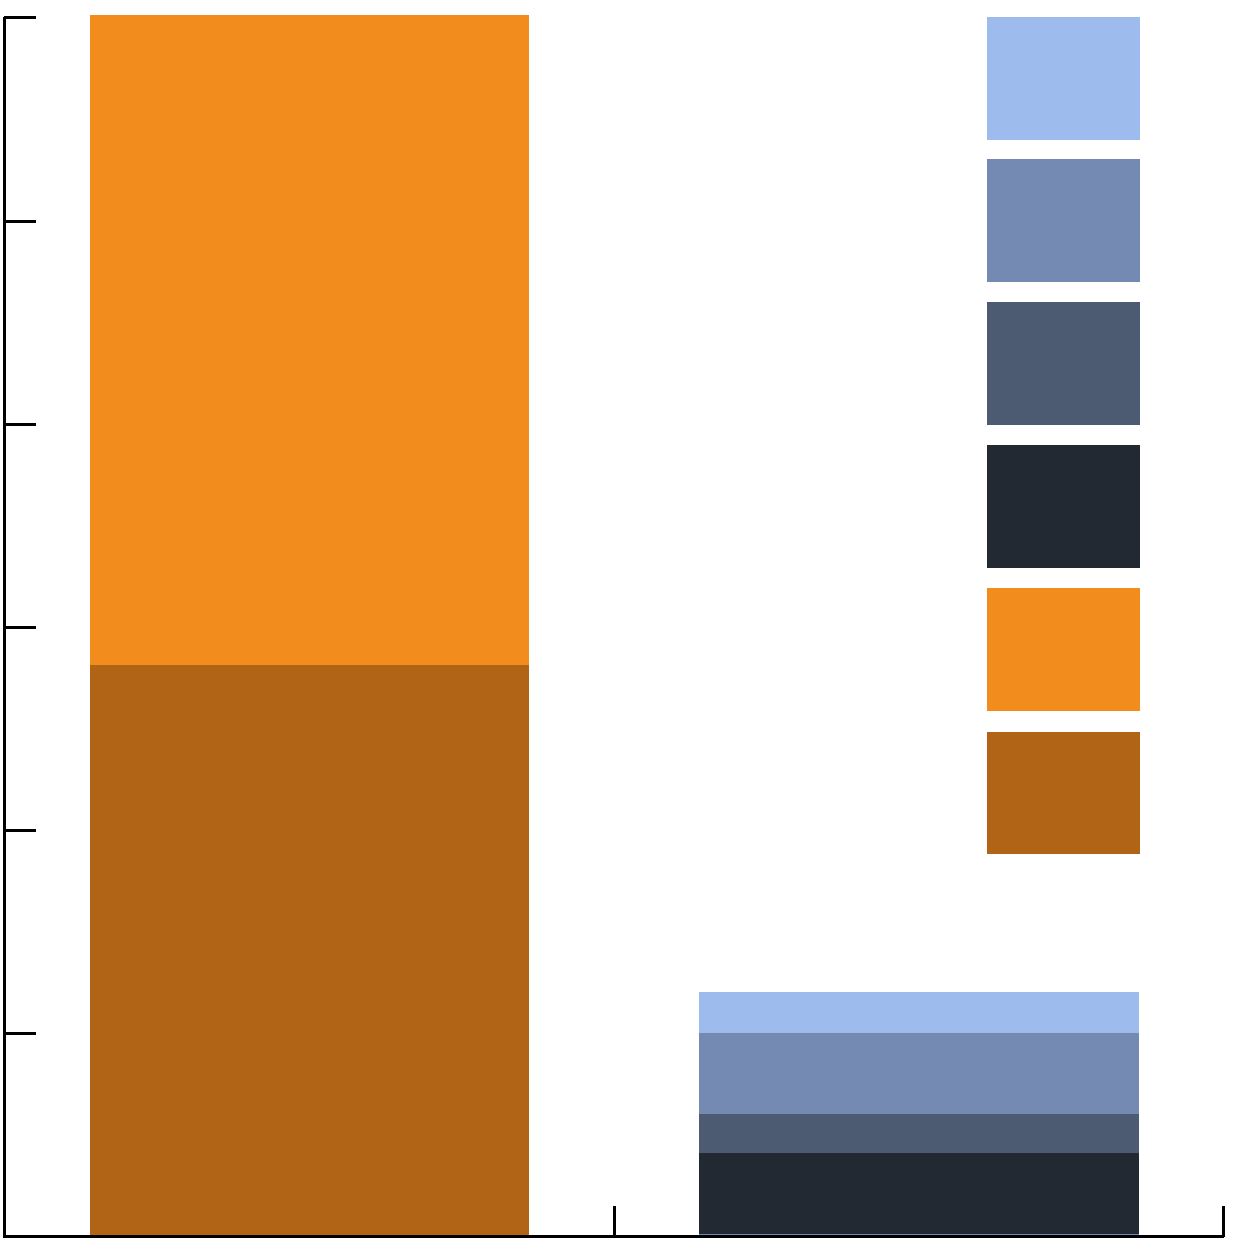
\includegraphics[width=60mm]{img/requirements-overview.pdf}};
	\begin{scope}[x={(image.south east)},y={(image.north west)}]
% 	% next four lines will help you to locate the point needed by forming a grid. comment these four lines in the final picture.↓
% 		\draw[help lines,xstep=.1,ystep=.1] (0,0) grid (1,1);
% 		\draw[help lines,xstep=.05,ystep=.05] (0,0) grid (1,1);
% 		\foreach \x in {0,1,...,9} { \node [anchor=north] at (\x/10,0) {0.\x}; }
% 		\foreach \y in {0,1,...,9} { \node [anchor=east] at (0,\y/10) {0.\y};}
% 	% upto here↑
	
	\draw (0.255,-0.040) node {\small \textsf{Functional}};
	\draw (0.744,-0.040) node {\small \textsf{Non-Functional}};
	
	\draw (-0.044,0.985) node {\small \textsf{30}};
	\draw (-0.044,0.820) node {\small \textsf{25}};
	\draw (-0.044,0.658) node {\small \textsf{20}};
	\draw (-0.044,0.494) node {\small \textsf{15}};
	\draw (-0.044,0.329) node {\small \textsf{10}};
	\draw (-0.034,0.168) node {\small \textsf{5}};
	\draw (-0.034,0.007) node {\small \textsf{0}};



	\draw (0.950,0.935) node[anchor=west] {\small \textsf{Backend}};
	\draw (0.950,0.820) node[anchor=west] {\small \textsf{Conventional}};
	\draw (0.950,0.705) node[anchor=west] {\small \textsf{Testing}};
	\draw (0.950,0.590) node[anchor=west] {\small \textsf{\acrshort*{UI}}};
	\draw (0.950,0.475) node[anchor=west] {\small \textsf{\acrshort*{UX}}};
	\draw (0.950,0.360) node[anchor=west] {\small \textsf{Feature}};
	
	\end{scope}
	\end{tikzpicture}
	\caption[Requirements Overview by Category]{Overview for functional (\textit{n}\,=\,30) and non-functional (\textit{n}\,=\,6) requirements by their category.}
	\label{fig:Requirements Overview}
	\libertineOsF
\end{figure}


\noindent Nevertheless, the other non-functional categories (i.e., \textit{\acrshort*{UI}, \textit{Testing}, \textit{Conventional}, and \textit{Backend}}) describe elements that are significant for the development process; most prominently, the integration into an existing infrastructure (\tracknshrink{NFR}\textsubscript{6}).

Overall, the listed requirements set a framework for a prototypical application state. The priority of functional requirements, however, have more significance compared to non-functional requirements. The requirement levels for most items are either \textit{\tracknshrink{MUST}} or \textit{\tracknshrink{SHOULD}}, as can be seen in \autoref{tab:RequirementLevel}. 


\begin{table}[H]\centering
\libertineLF
\begin{tabular}{lccccc} \toprule
Category & \multicolumn{5}{c}{Requirement Levels} \\\cmidrule(rl){2-6}
& \tracknshrink{MUST} & \tracknshrink{SHOULD} & \tracknshrink{MAY} & \tracknshrink{SHOULD NOT} & \tracknshrink{MUST NOT} \\\midrule
Feature         & 9 & 2 & 1 & 1 & 1 \\
\acrshort*{UX}  & 12 & 4 & - & - & - \\\addlinespace

\acrshort*{UI}  & 2 & - & - & - & - \\
Testing         & - & 1 & - & - & - \\
Conventional    & - & 2 & - & - & - \\
Backend         & 1 & - & - & - & - \\\midrule

Functional      & 21 & 6 & 1 & 1 & 1 \\
Non-Functional  & 3 & 3 & - & - & - \\\midrule

Sum             & 24 & 9 & 1 & 1 & 1 \\\bottomrule
\end{tabular}
\caption[Requirements Overview by Requirement Level]{Requirements overview by their requirement level \parencite[see][]{Bradner1997}.}
\label{tab:RequirementLevel}
\libertineOsF
\end{table}

\noindent There is only one requirement that must not be specified, that is the ability to drop cards on adjacent lanes (see \tracknshrink{FR}\textsubscript{5}). Moreover, the subject of column and lane order and repositioning (as outlined in \tracknshrink{FR}\textsubscript{6}) has a level of \textit{\tracknshrink{SHOULD NOT}}, since it requires further research (as described in \autoref{ch:Discussion}).